\section{Текущая модель организации антинаркотического мониторинга и анализа
наркоситуации на региональном уровне на примере Санкт-Петербурга}

Мониторинг и анализ наркоситуации на данный момент являются одними из самых
актуальных вопросов Государственной антинаркотической политики и деятельности по
противодействию незаконному обороту наркотиков и распространению наркомании. 

В Санкт-Петербурге мониторинг наркоситуации осуществляется с 2003 года. На
основе ранее организованного комплексного мониторинга социально-экономического
развития города – как субъекта Федерации, на первом этапе  анализировалось
исполнение мероприятий целевых программ Санкт-Петербурга по противодействию
злоупотреблению наркотиками и их незаконному обороту.

В настоящее время целевое предназначение мониторинга гораздо шире. С одной
стороны – это информационно-аналитическая поддержка процесса формирования
надведомственных решений, обеспечивающих выполнение государственной
антинаркотической политики на территории субъекта, а с другой – информационное
обеспечение на уровне каждого ведомства, решающего обозначенную проблему с
учетом деятельности других ведомств.

Правовой основой организации мониторинга наркоситуации, последовательного
создания межведомственной Базы данных, а затем АИС мониторинга является
Стратегия государственной антинаркотической политики, а также Постановление
правительства Российской Федерации «Об утверждении Положения о государственной
системе мониторинга наркоситуации в Российской Федерации».

На уровне региона вступило в силу Постановление Губернатора Санкт-Петербурга от
20.09.2012 N 60-пг "О мониторинге наркоситуации в Санкт-Петербурге".

\textit{Автоматизированные средства проведения мониторинга наркоситуации}.
В Санкт-Петербурге мониторинг наркоситуации осуществляется с применением
автоматизированной информационной системы, являющейся по сути
информационно-аналитической системой АИС «Антинар СПб».

АИС «Антинар СПб» - автоматизированная система, ориентированная  на комплексный
анализ наркоситуации во всех сферах  жизнедеятельности города, выявление
важнейших тенденций и закономерностей ее развития, информационно-аналитическую
поддержку процесса принятия управленческих решений руководством
Санкт-Петербурга.

Среди основных задач, решаемых за счет автоматизации процессов мониторинга,
анализа и прогнозирования выделяют:
\begin{itemize}
\item сбор, предварительная обработка, структурирование, интеграция и хранение
информации о наркоситуации (фильтрация, проверка на полноту и достоверность,
верификация, резервирование, восстановление и т.д.);
\item поддержание в актуальном состоянии Базы данных (БД АИС «Антинар СПб»),
содержащей разностороннюю информацию о наркоситуации в Санкт-Петербурге;
аналитическая обработка информации, решение расчетных задач, получение
агрегированных текущих и прогнозных оценок развития наркоситуации в городе на
основе применения современных информационных технологий;
\item моделирование и прогнозирование процессов наркоситуации в Санкт-Петербурге;
разработка предложений для принятия соответствующих управленческих решений;
анализ исполнения мероприятий целевых программ по противодействию
злоупотреблению наркотиками и их незаконному обороту;
\item информационно-аналитическая и информационно-справочная поддержка
управленческой деятельности руководства города.
\end{itemize}
Таким образом, основное предназначение АИС «Антинар СПб» –
информационно-аналитическая поддержка процесса принятия управленческих решений
Губернатором Санкт-Петербурга, Правительством Санкт-Петербурга, руководителями
ИОГВ по определению приоритетных направлений антинаркотической деятельности в
Санкт-Петербурге. 

Создание межведомственного информационного ресурса:
\begin{itemize}
\item определение круга отраслевых и территориальных структур (ведомств),
осуществляющих деятельность по противодействию злоупотреблению наркотиками и их
незаконному обороту и  разработку Положения об информационном взаимодействии
между ними в процессе мониторинга;
\item разработка, согласование и утверждение Перечня показателей наркоситуации и
Регламента подготовки и представления данных в единую базу данных (БД). 
\end{itemize}
Перечень составляют показатели по различным направлениям мониторинга
наркоситуации: незаконный оборот наркотиков, наркомания, окружающая среда,
профилактика наркозависимости, показатели мониторинга наркоситуации в Российской
Федерации по методике ГАК. Наличие в Перечне показателей, относящихся к
районному уровню, позволяет осуществлять мониторинг наркоситуации с учетом
особенностей ее развития в районах города, там, где непосредственно проживают
группы риска населения, имеющие отношение к незаконному обороту наркотиков. 


В результате проделанной работы сформирована единая межведомственная База данных
по показателям наркоситуации, обеспечивающая возможность их анализа,
сопоставления и прогноза. 

Разработанный алгоритм мониторинга базируется на принципах использования единых
и обязательных для всех участников методологических подходов и критериев оценки
показателей наркотической ситуации, открытости используемых для мониторинга
данных, безвозмездного обмена информацией. Результат – возможность проводить на
уровне города комплексный объективный анализ динамики ситуации.

На втором этапе при тесном взаимодействии с Комитетом по вопросам законности,
правопорядка и безопасности и с Комитетом по информатизации и связи создана АИС
мониторинга наркоситуации «Антинар СПб», которая позволяет наблюдать и
анализировать срезы состояния тех или иных взаимоувязанных показателей по итогам
квартала, полугодия и года. Система реализована с учетом всех требований по
работе с конфиденциальной информацией и аттестована по классу 1Г. Сформирован
работоспособный коллектив специалистов по анализу данной предметной области.

Работа с данными по показателям наркоситуации, поступившим из разных ведомств,
позволяет не только увидеть картину в целом, но и выявлять скрытые процессы или
намечающиеся тенденции, изучать состояние и динамику наркоситуации, ее отдельные
составляющие, например:
\begin{itemize}
\item наркорынок; 
\item заболеваемость, в том числе по районам;
\item преступность, связанная с незаконным оборотом наркотиков и т.д.
\end{itemize}

\textit{Информационная поддержка принятия управленческих решений.}
Важнейшей характеристикой статистической информации, определяющей ее пригодность
для решения задач социального управления, является достоверность, под которой
понимается степень адекватности отображения информацией описываемых явлений,
событий или процессов. Достоверность данных в базе АИС «Антинар СПб»
обеспечивается документальным сопровождением и указанием источников всех
загружаемых значений.

Наличие межведомственной системы позволяет координировать деятельность
соответствующих исполнительных органов государственной власти с учетом
общегородских задач (рис. ~\ref{fig:org_mezhved_antinar}). Например,
модернизация системы учета больных в государственных наркологических учреждениях
здравоохранения или профилактических программ, осуществляемых заинтересованными
в решении своих проблем администрациями  районов.

\begin{figure}
    \centering
    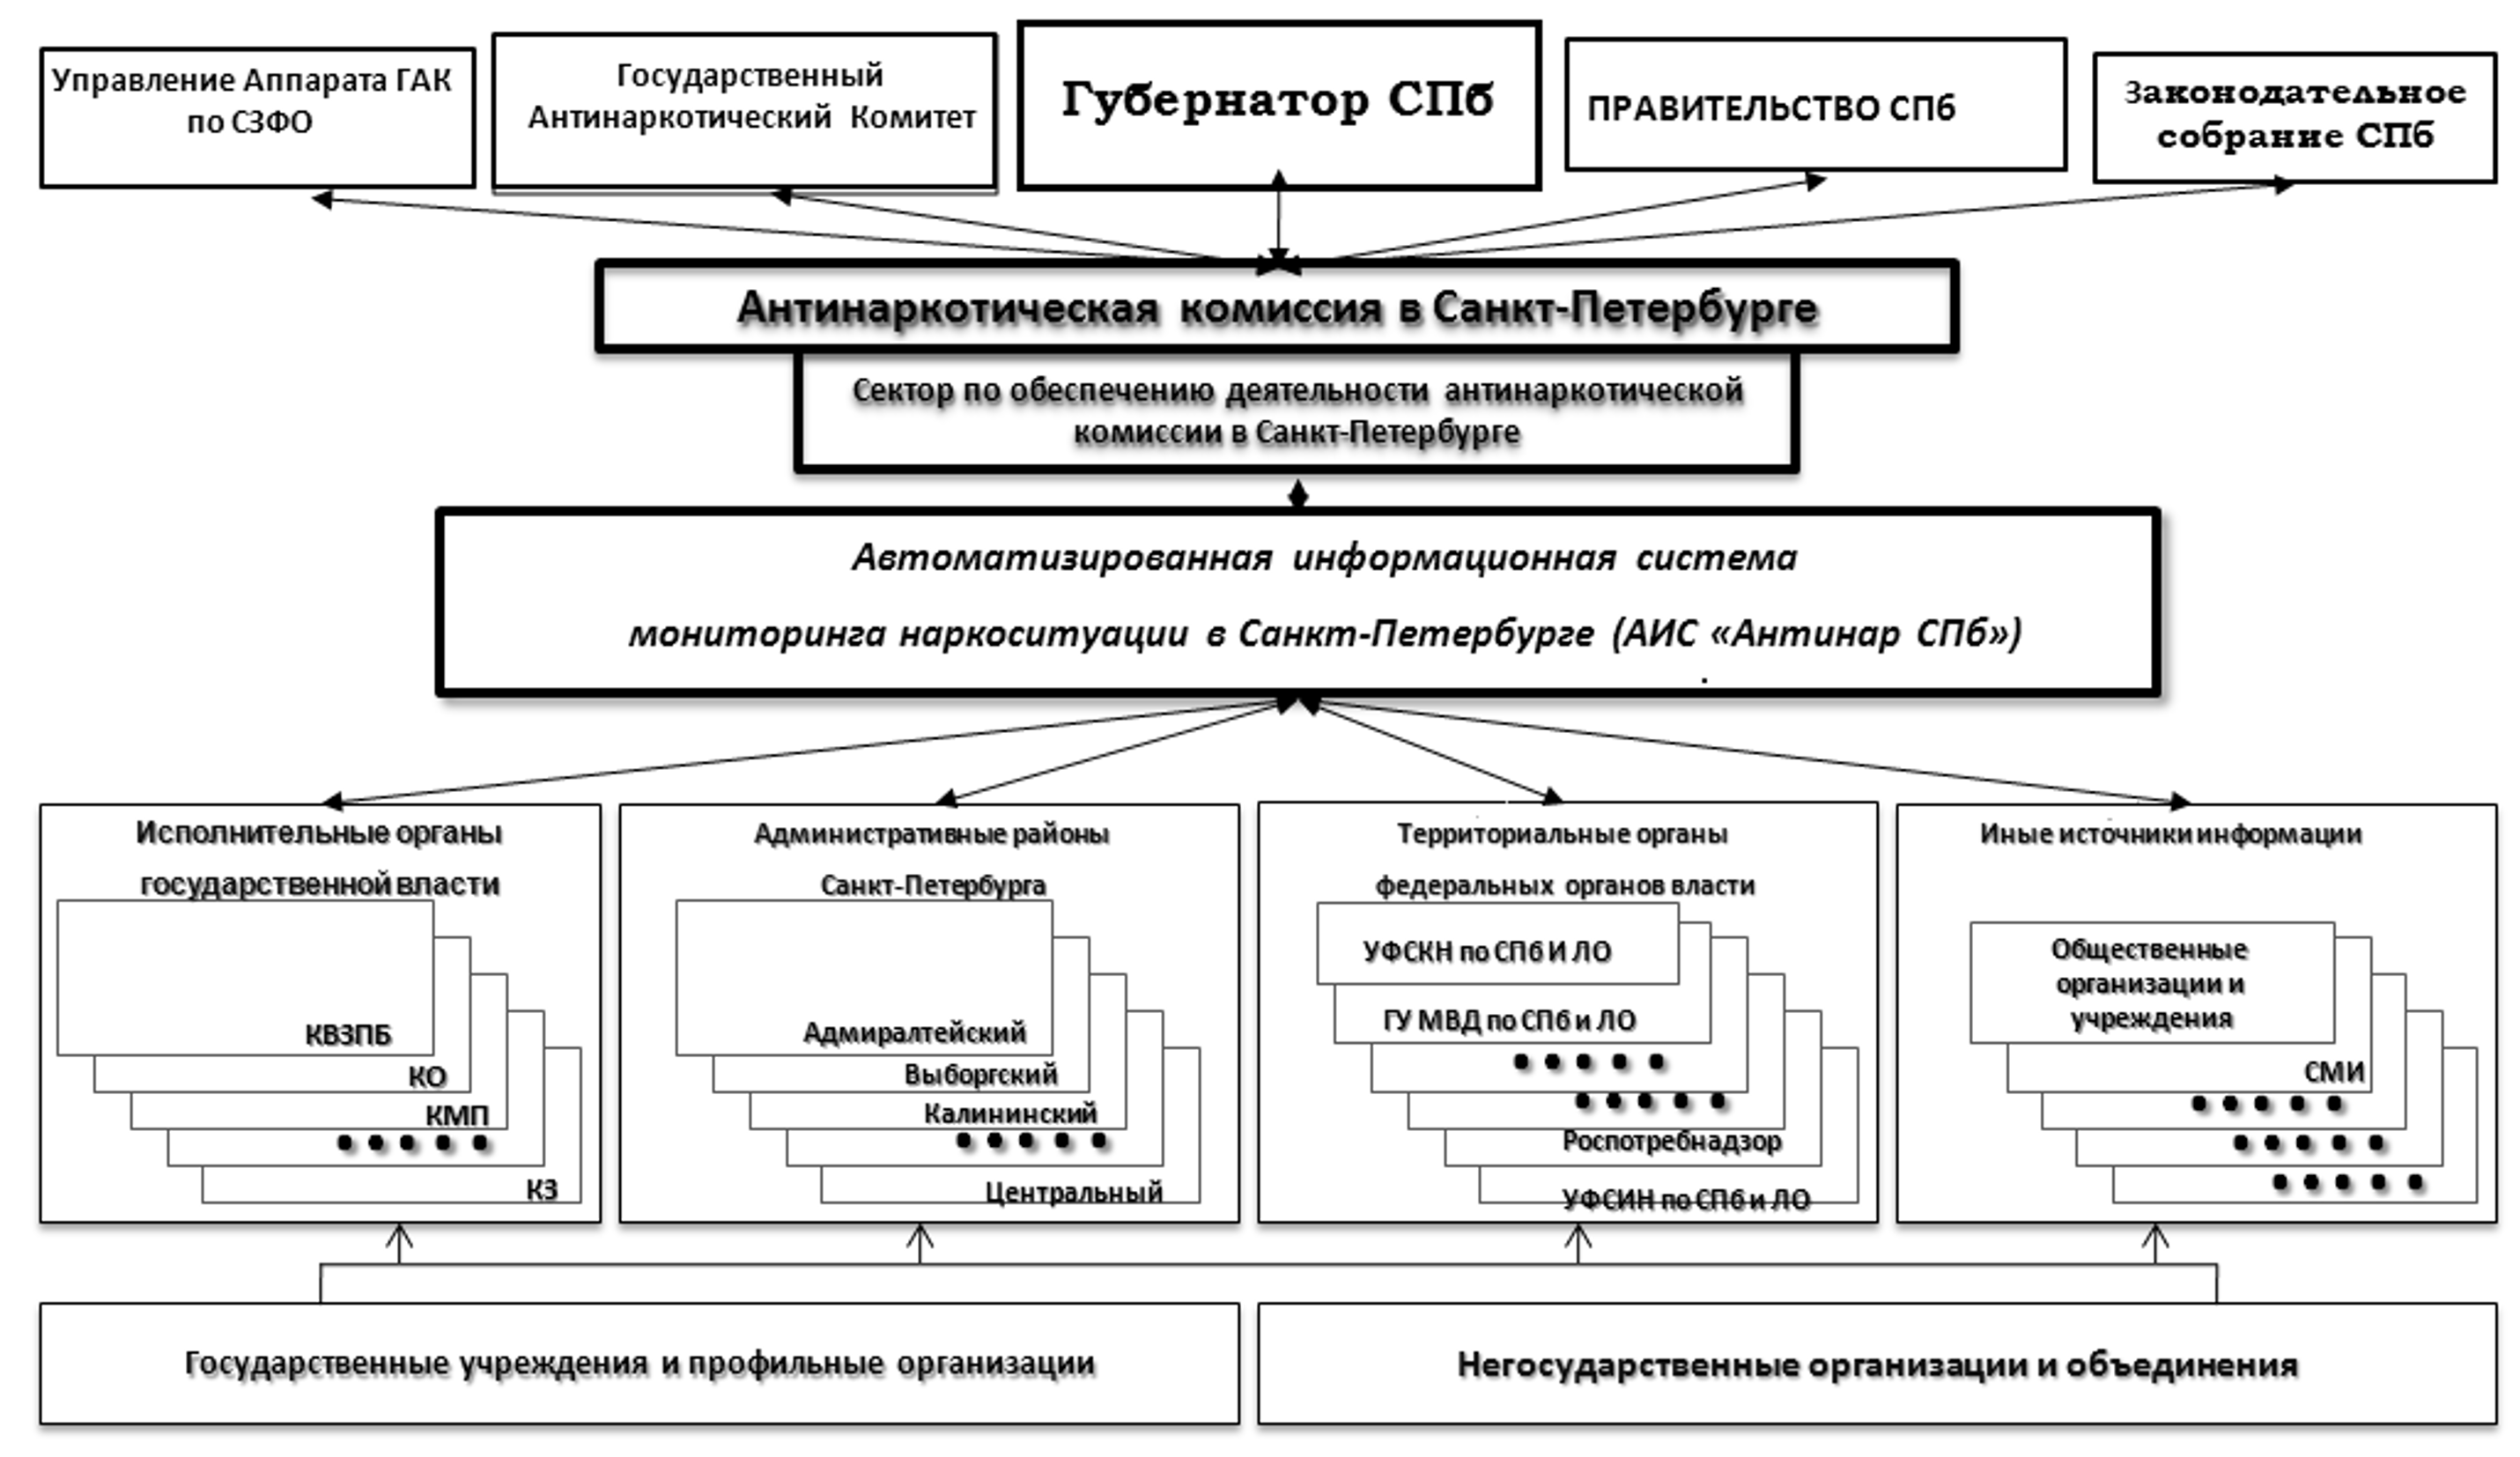
\includegraphics{org_mezhved_antinar.png}
    \caption{Организация межведомственного мониторинга наркоситуации с
    использованием АИС «Антинар СПб»}
    \label{fig:org_mezhved_antinar}
\end{figure}

Комплексный анализ наркоситуации на средствах АИС «Антинар СПб» включает:
\begin{itemize}
\item анализ динамики и прогнозирование  процессов  распространения и последствий
незаконного оборота наркотиков;
\item оценку влияния наркоситуации на социально-экономические аспекты
жизнедеятельности города;
\item оценка численности потребителей психоактивных веществ, неучтенных в
официальной статистике (Оценка величины латентности);
\item оценка кризисности наркоситуации в регионе на основе латентностных
характеристик;
\item анализ выполнения целевых программ по противодействию злоупотреблению
наркотиками и их незаконному обороту.
\end{itemize}

Злоупотребление психоактивными веществами является сложным социальным процессом,
скрытым от непосредственного наблюдения и оценивания. Поэтому его
распространение нельзя ограничивать только фиксированным перечнем статистических
показателей, учитываемых государственной и ведомственной статистикой. В силу
специфики проблемы наркотизации населения, прежде всего ее высокой латентности,
классические методы изучения ведомственной статистики недостаточны для
объективной оценки состояния наркообстановки. Поэтому обязательной составляющей
мониторинга являются данные социологических исследований и экспертных оценок  по
целому ряду вопросов наркоситуации.

В связи с этим следует отметить, что в городе до настоящего времени не сложилась
система комплексного учета данных тематических оценочных исследований,
проводимых государственными структурами и общественными организациями или
фондами  в различных слоях общества и по сути своей мониторирующих происходящие
в обществе процессы. Никто из специалистов  ИОГВ не может точно сказать кто,
сколько, как и зачем исследует на подведомственных им территориях, какие
результаты получает и как их использует в дальнейшем. А ведь только объединение
усилий государства и общества обеспечит успех в противодействии наркомании. Эта
проблема требует своего решения в рамках обсуждаемого мониторинга.

\textit{АИС «Антинар СПб» как региональный сегмент государственной системы
мониторинга наркоситуации в Российской Федерации}
Согласно постановлению Правительства №485, методике мониторинга
наркоситуации ГАК и приложениям к ней определен порядок мониторинга по
показателям наркоситуации на региональном и федеральном уровне. Согласно данным
постановлениям, в базе данных АИС «Антинар СПб» создан раздел «Мониторинг
наркоситуации по методике ГАК». Тем самым АИС «Антинар СПб»
является региональным сегментом государственной системы мониторинга
наркоситуации в Российской Федерации.

На основе программно-технических средств АИС «Антинар СПб» организовано
функционирование единой базы данных по вопросам наркоситуации в субъектах СЗФО в
рамках организации мониторинга наркоситуации на территории СЗФО согласно
методике ГАК. С этой целью реализовано:
\begin{enumerate}
\item создано программно-техническое ядро единой БД.
\item в единой БД «Антинар СПб – СЗФО» размещены:
\begin{itemize}
\item показатели мониторинга наркоситуации согласно приложениям №№ 1-53 к методике
мониторинга наркоситуации ГАК; 
\item данные по показателям для оценки степени тяжести наркоситуации в субъектах
 СЗФО.
\end{itemize}
\end{enumerate}
 Источниками информации являются исполнительные органы государственной
 власти и органы местного самоуправления субъектов СЗФО и УФСКН субъектов СЗФО. 
 Передача данных с мест на первом этапе может обеспечиваться по электронной
 почте, на бумажных носителях, либо с помощью разработанного типового модуля.
 При этом информационные потоки в предлагаемом формате и с установленной
 периодичностью будут поступать из регионов СЗФО в Единую БД АИС «Антинар СПб -
 СЗФО».

\begin{figure}
    \centering
    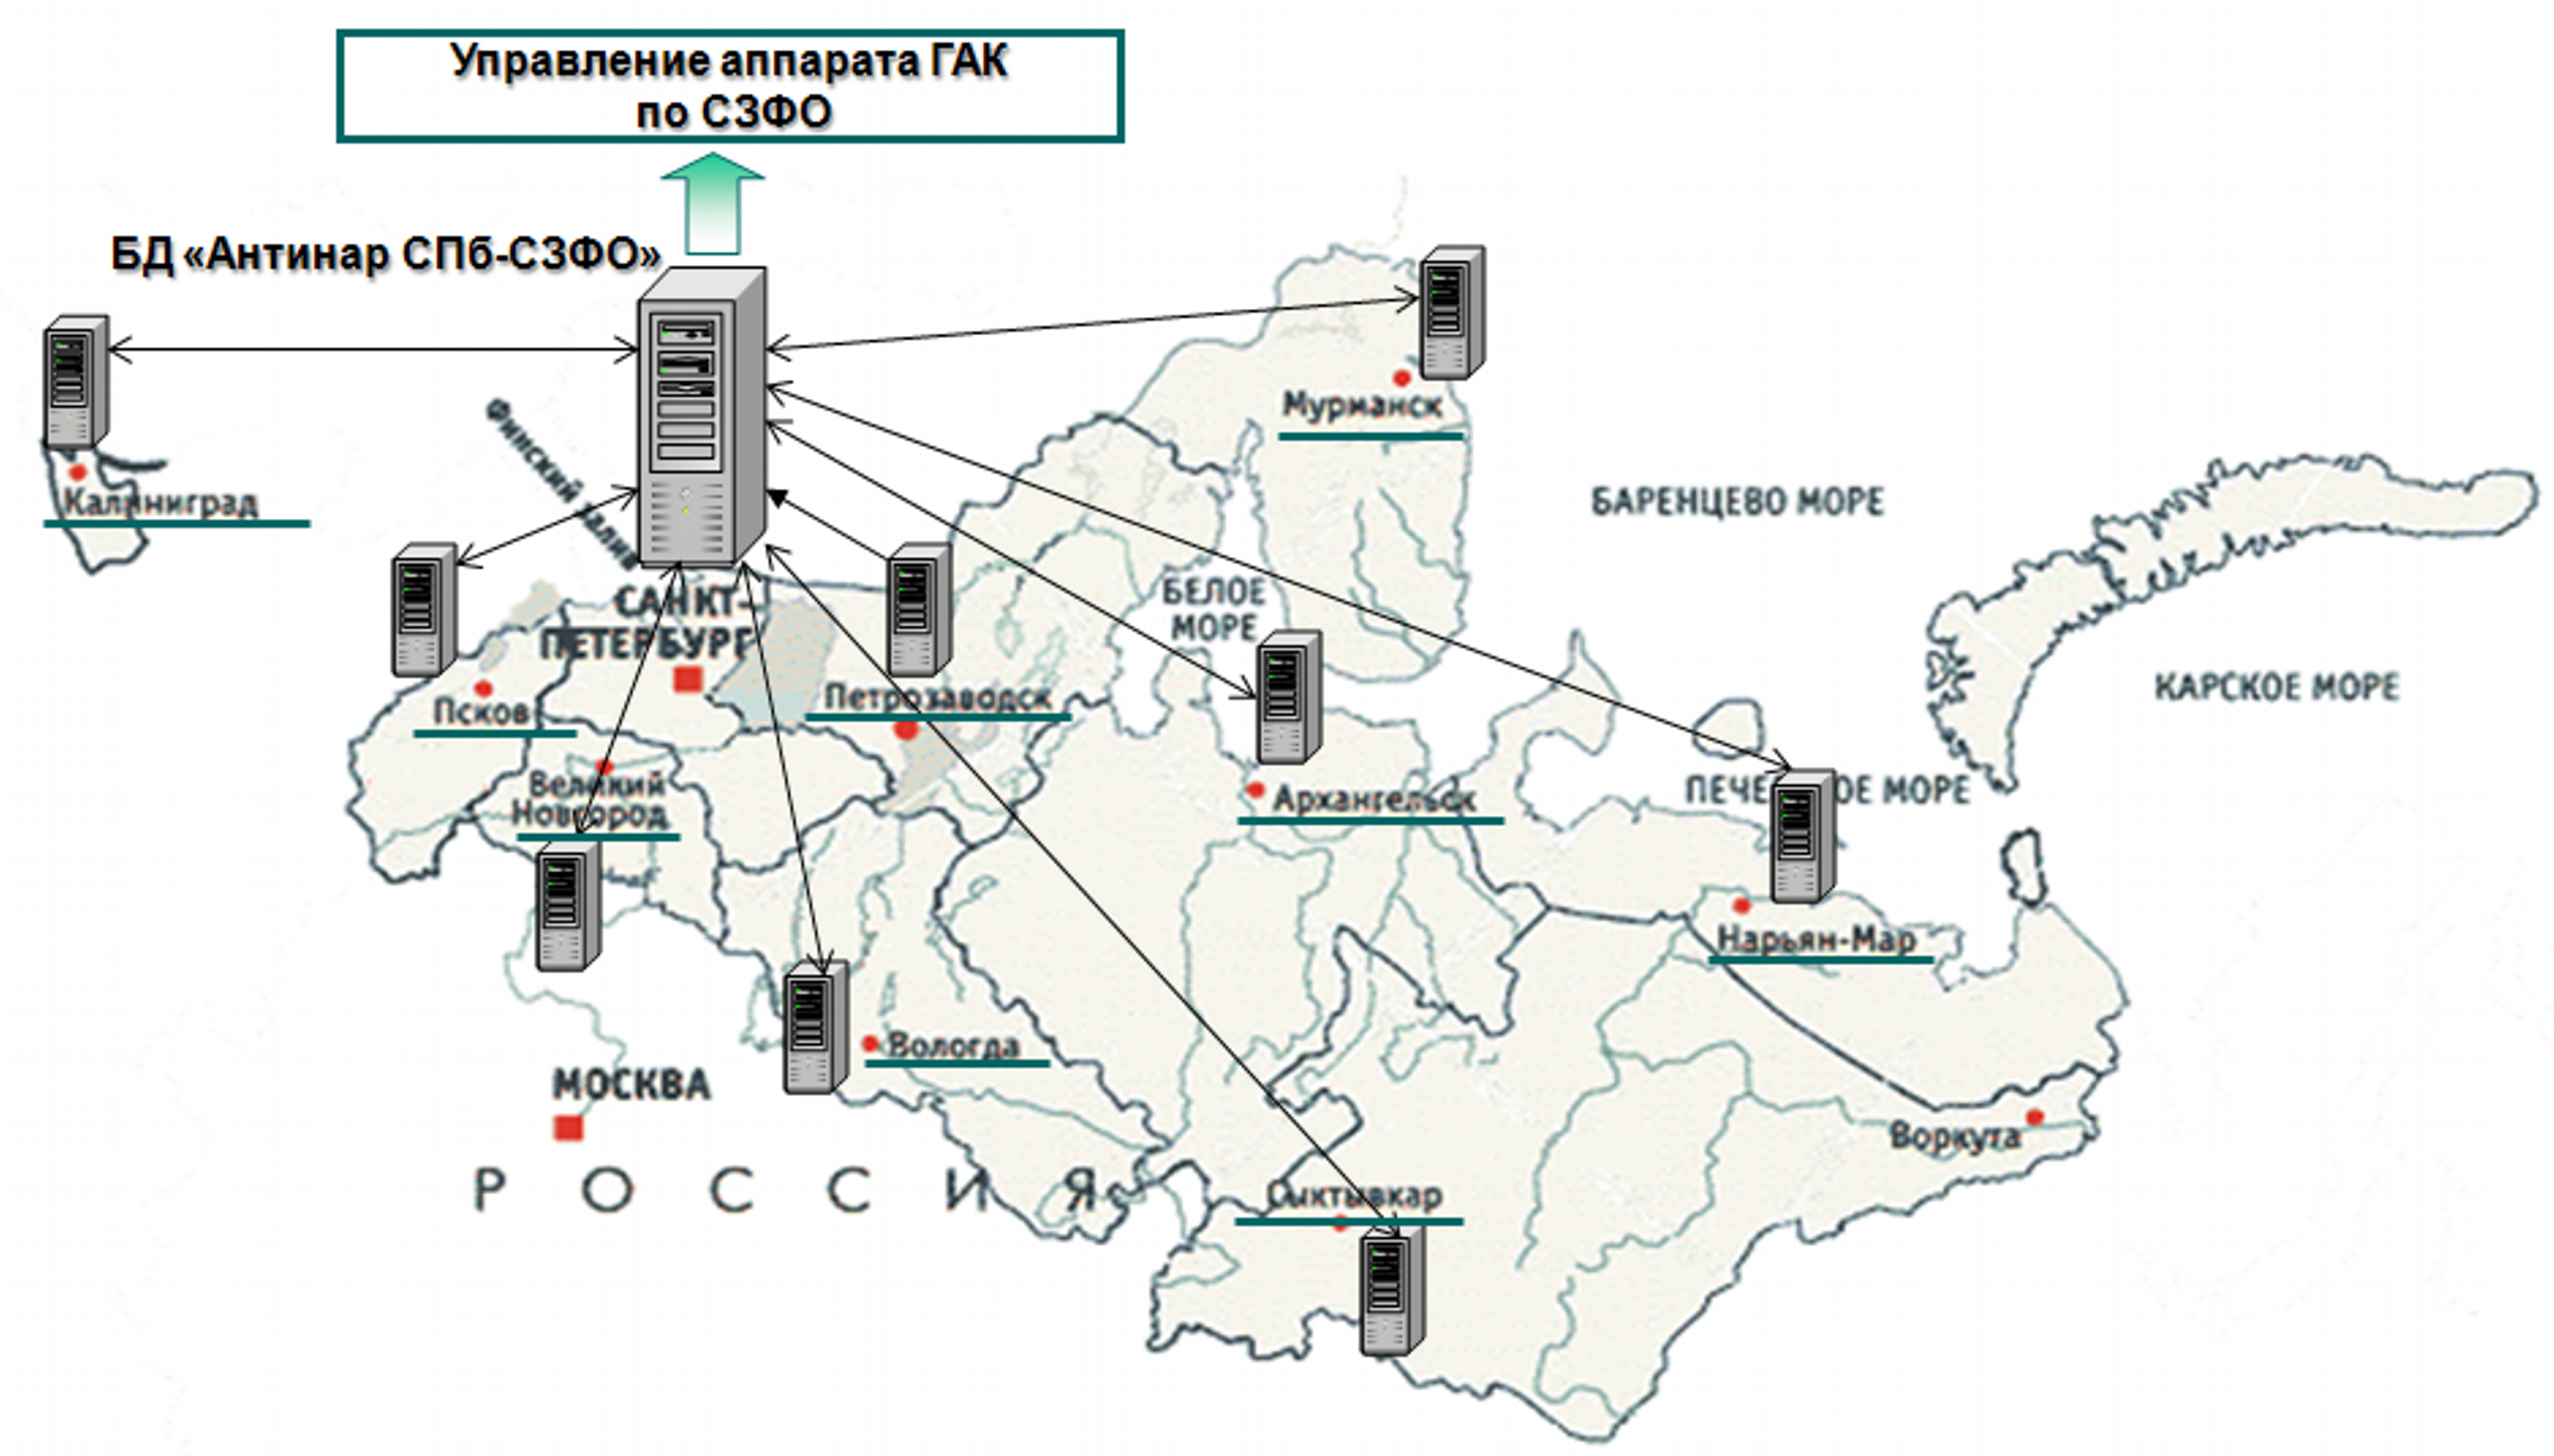
\includegraphics{gak_sfzo_monitoring.png}
    \caption{Схема формирования информационно-коммуникационной основы
    мониторинга наркоситуации в СФЗО}
    \label{fig:gak_sfzo_monitoring}
\end{figure}

\textit{Геоинформационный сегмент АИС «Антинар СПб»}
В геоинформационном сегменте АИС «Антинар СПб» рассматривается анализ
информации, имеющей жесткую привязку к географическим. В АИС «Антинар
СПб» представлены ГИС-слои по направлениям:
\begin{enumerate}
\item мониторинг сообщений населения о местах распространения наркотиков по
телефонам горячей линии;
\item мониторинга деятельности ФСКН – места задержаний распространителей
наркотиков, лабораторий и пр.;
\item мониторинг токсикологической ситуации, включая места отравлений
наркотическими средствами и психотропными веществами, отравлений с целью
опьянения и пр.;
\item мониторинг профилактической деятельности в Санкт-Петербурге, включая места
проведения мероприятий антинаркотической направленности;
\item и другие слои, включающий сопутствующую информацию о территории.
\end{enumerate}

Достоинством данного подхода является его наглядность и простота восприятия, а
также жесткая привязка к реальным объектам, что упрощает интерпретацию
результатов и выработку управленческих решений. Вследствие описанных
особенностей рассматриваемые методы применимы в задаче оценки эффективности
работы с населением, в частности, в задаче организации мероприятий первичной
профилактики. Организация профилактической работы подразумевает определение
места проведения и целевую аудиторию ряда мероприятий, что позволяет
осуществлять ее анализ посредством ГИС. 

\textit{Портал «Антинаркотическая политика в Санкт-Петербурге».} Пространство
Интернет является важнейшим ресурсом, посредством которого реализуется масса
различных информационно-пропагандистских мероприятий. Поэтому особенно ценной,
на наш взгляд, явилась возможность освещения государственной антинаркотической
политики со страниц интернет-сайта.  

Поскольку информационные ресурсы базы данных Автоматизированной информационной
системы мониторинга наркоситуации в Санкт-Петербурге (АИС «Антинар СПб»),
информационно-аналитические материалы, разработанные на инструментальных
средствах системы доступны только для руководителей и специалистов ИОГВ (система
защиты информации АИС классифицирована по классу 1Г), то возникла необходимость
в создании информационного инструмента для более широкого круга пользователей.
Это и обусловило создание сайта. 

В рамках решения задачи организации электронного правительства по направлению
создания сети сайтов и порталов, направленных на иллюстрацию деятельности
органов государственной власти населению в Интернет, разработан и функционирует
интернет-ресурс «Антинаркотическая политика в Санкт-Петербурге».

Главная цель создания данного сайта – объективное и полное отражение
государственной антинаркотической политики, реализуемой исполнительными органами
государственной власти на территории Санкт-Петербурга и его районов,
формирование у широкого круга пользователей сайта представления о деятельности
ИОГВ и их возможностях в области противодействия злоупотреблению наркотическими
средствами и их незаконному обороту.

Сайт позволяет избежать длительных процедур ознакомления с деятельностью органов
власти в поисках тематической информации по противодействию распространению
наркозависимости. Сайт дает возможность предоставления любому заинтересованному
контингенту пользователей документов, фотоматериалов и другой информации в
больших объемах и с высокой оперативностью. 

С помощью сайта можно мгновенно известить большое количество пользователей о
главных мероприятиях и важнейших событиях антинаркотической деятельности в
Санкт-Петербурге и его районах.

С учетом практически неограниченного охвата аудитории мы получили мощное и
эффективное информационно-пропагандистское средство, несущее пользователям
актуальную информацию о деятельности отраслевых и территориальных ИОГВ
Санкт-Петербурга по реализации государственной антинаркотической политики. 
Одной из главных задач сайта является обеспечение координации деятельности
территориальных органов исполнительной власти и антинаркотических комиссий в
районах Санкт-Петербурга, а также организация их взаимодействия между собой, с
органами исполнительной власти города, органами местного самоуправления
муниципальных образований, общественными объединениями и организациями.

\textit{Методологические подходы к анализу наркоситуации.}
Для комплексной оценки наркоситуации в системе реализован известный методический
подход, основанный на сопоставлении значения того или иного индикативного
показателя наркоситуации с устанавливаемым для него пороговым (нормативным)
уровнем. Это позволяет определять степень кризисности ситуации, складывающейся в
регионе (рис. ~\ref{fig:antinar_methodology}). 

Анализ наркоситуации по данной методике позволяет дать оценку социальной
стоимости ущерба от распространения наркомании, количеству наркозависимых на
территории, числу лиц, занимающихся незаконным оборотом наркотиков, уровню
преступности в сфере незаконного оборота наркотиков, уровню наркотизации
различных групп населения (женщины, подростки) и демографической устойчивости
территории, а также выйти на интегральную оценку наркоситуации в регионе. 

\begin{figure}
    \centering
    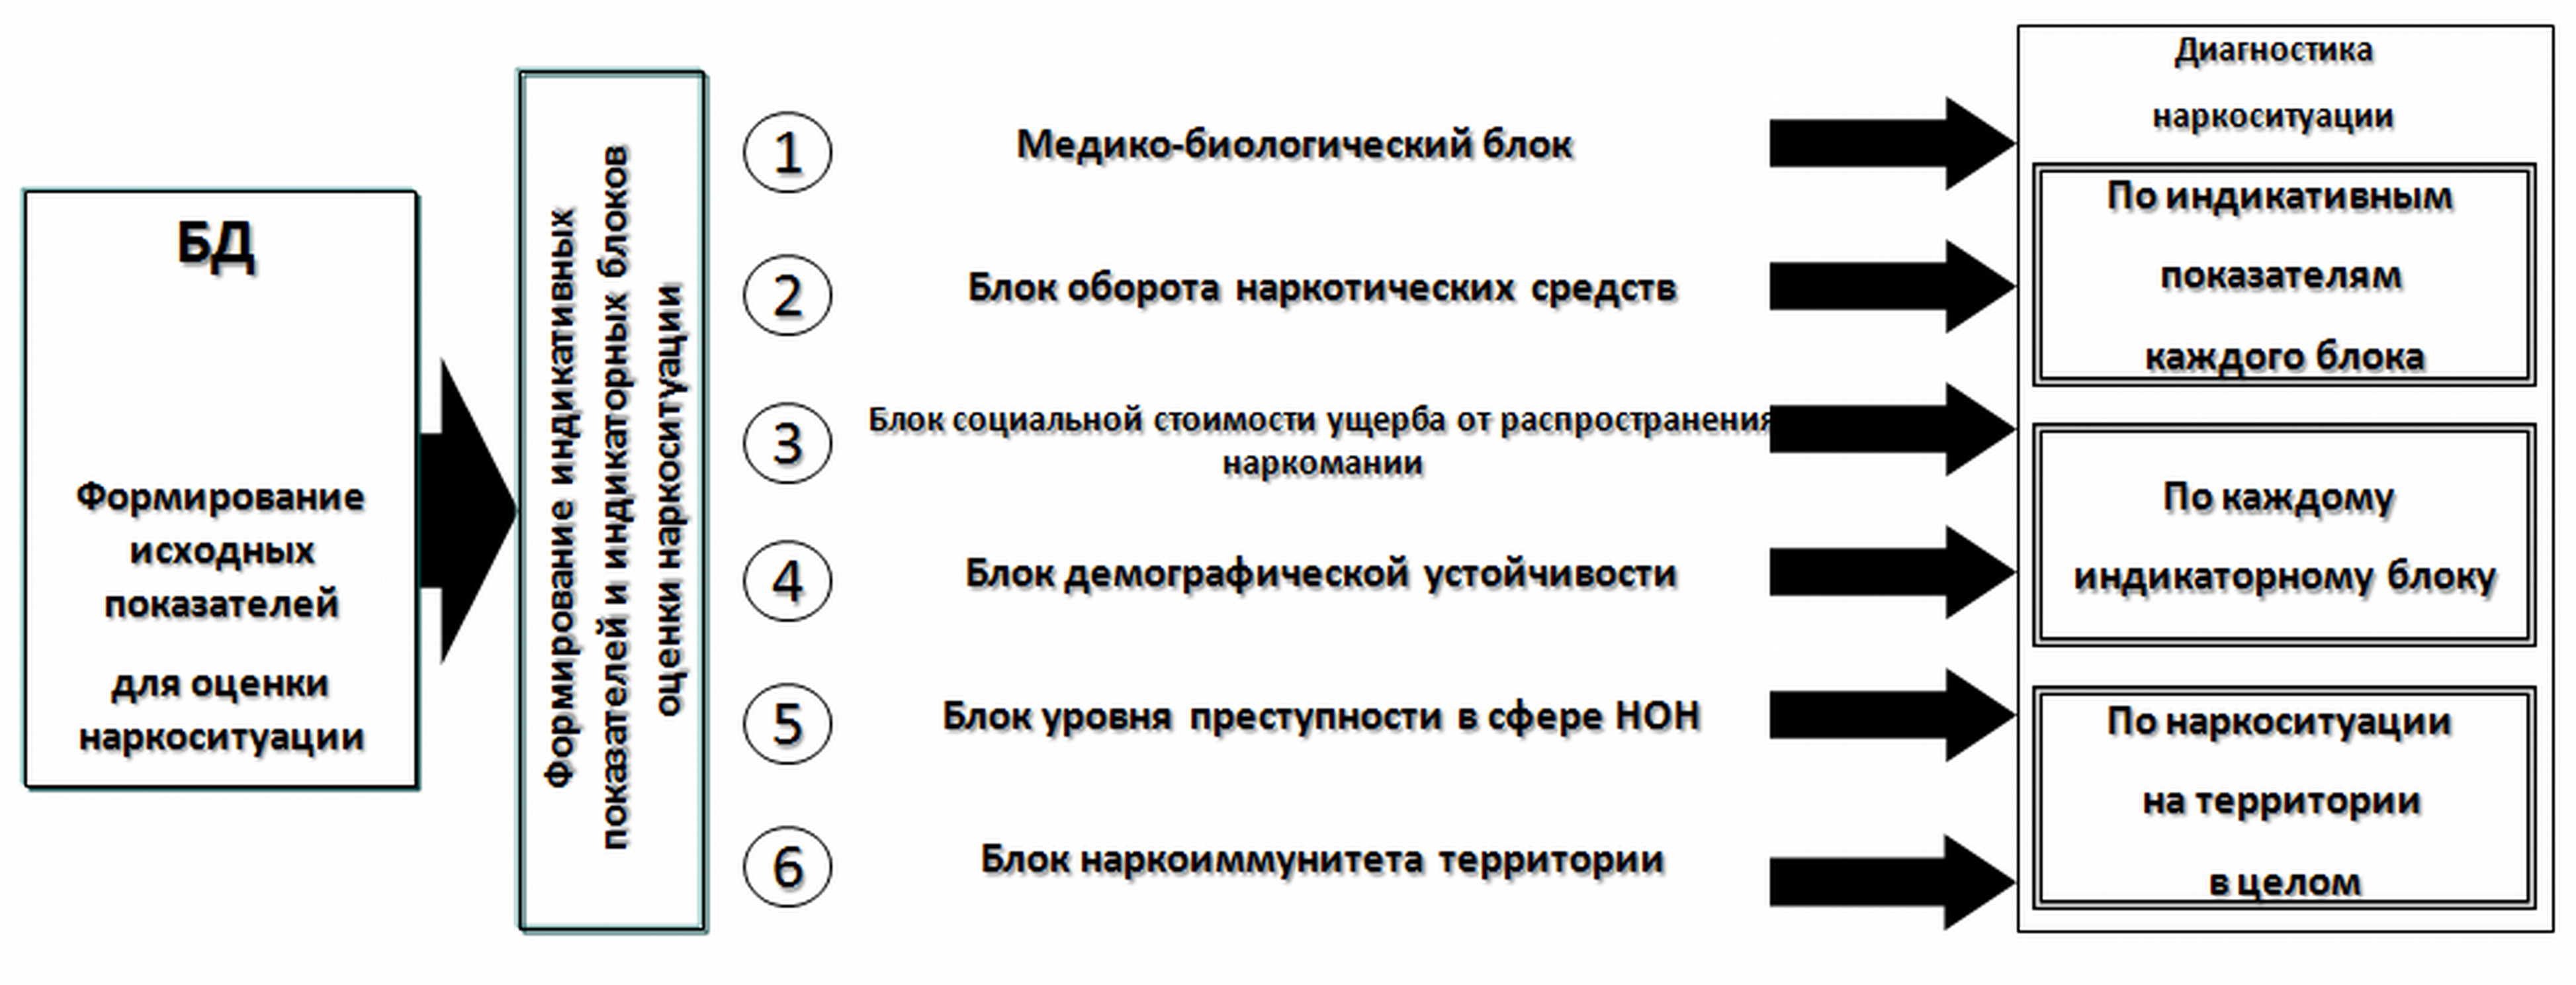
\includegraphics[width=\textwidth]{antinar_methodology.png}
    \caption{Методические основы анализа наркоситуации с использованием АИС
    «Антинар СПб»}
    \label{fig:antinar_methodology}
\end{figure}

По каждому блоку индикативных показателей производится оценка пороговых уровней
наркоситуации. В используемой методике определения пороговых значений
индикативных показателей мы исходили из положений о демографической безопасности
территории. Под демографической безопасностью понимаем состояние защищенности
общества, проживающего на территории, его образа жизни, культурно-исторического
наследия и др. Именно сохранение коренного населения территории мы видим
основной целью мероприятий укрепления национальной безопасности, в частности
борьбы с распространением наркозависимости.

Следует отметить, что использование пороговых уровней показателей наркоситуации
позволяет получить нижнюю оценку кризисности наркоситуации, таким образом,
возникает дополнительная задача определения оптимального направления
деятельности по ликвидации кризисности наркоситуации.

Пороговые значения показателей служат для оценки степени кризисности ситуации в
рассматриваемой сфере. В литературе встречается определение уровней
кризисности порогов индикаторов как степеней угроз нормальному функционированию
системы. Предполагается, что по выбранному перечню индикативных показателей
должны быть определены некие критические значения, в случае превышения которых
следуют изменения, требующие оперативного вмешательства в рассматриваемый
процесс. Нами рассматривается следующая система пороговых уровней:
\begin{itemize}
\item[] ПК1 – предкризисное состояние первого уровня, характеризуется ожиданием
наступления кризиса с 95\% вероятностью в течение пяти лет;
\item[] ПК2 – предкризисное состояние второго уровня, характеризуется ожиданием
наступления кризиса с 95\% вероятностью в течение трех лет;
\item[] ПК1 – кризисное состояние, характеризуется наличием явных угроз демографической
безопасности региона;
\item[] ПК2 – кризисное состояние второго уровня, характеризуется завершающей стадией
эпидемического процесса развития наркомании и значительной угрозой
демографической безопасности региона;
\item[] ПК3 – кризисное состояние третьего уровня, характеризуется практическим
уничтожением этноса, массовым оттоком коренного населения, замещением населения
трудовыми мигрантами.
\end{itemize}

Отнесение ситуации в регионе к какому-либо из перечисленных состояний аналогична
проверке гипотезы наличия в регионе кризисной ситуации. Уменьшение вероятностей
ошибок первого и второго рода в данном случае достигается за счет выбора
соответствующего критерия отнесения ситуации к соответствующему состоянию. 

В данной методике определение пороговых уровней опирается на величину
латентности наркоситуации. Основное положение состоит в том, что реальное число
наркозависимых не должно превысить определенного критического значения, когда
развитие наркомании приведет к деградации общества и развалу экономики региона.
Таким образом, определение пороговых уровней учитывает необходимость снижения
фактической преступности и заболеваемости в сфере незаконного оборота
наркотиков, а также уменьшение теневой доли данных процессов.

\textit{Прогнозирование наркоситуации в Санкт-Петербурге}
Прогнозирование наркоситуации является важнейшей составляющей деятельности в
сфере информационной поддержки принятия управленческих решений, поскольку
позволяет не только оценить эффективность принимаемых мер противодействия, но и
моделировать развитие наркоситуации в зависимости от сценария противодействия с
целью нахождения наилучшего решения.

Получение прогноза требует разработки специфических подходов в силу скрытого
характера явления наркомании. Для организации эффективных мер противодействия
существует необходимость прогнозировать развитие наркоситуации в зависимости от
общей социальной, экономической, психологической и политической  обстановки на
территории.

\begin{figure}
    \centering
    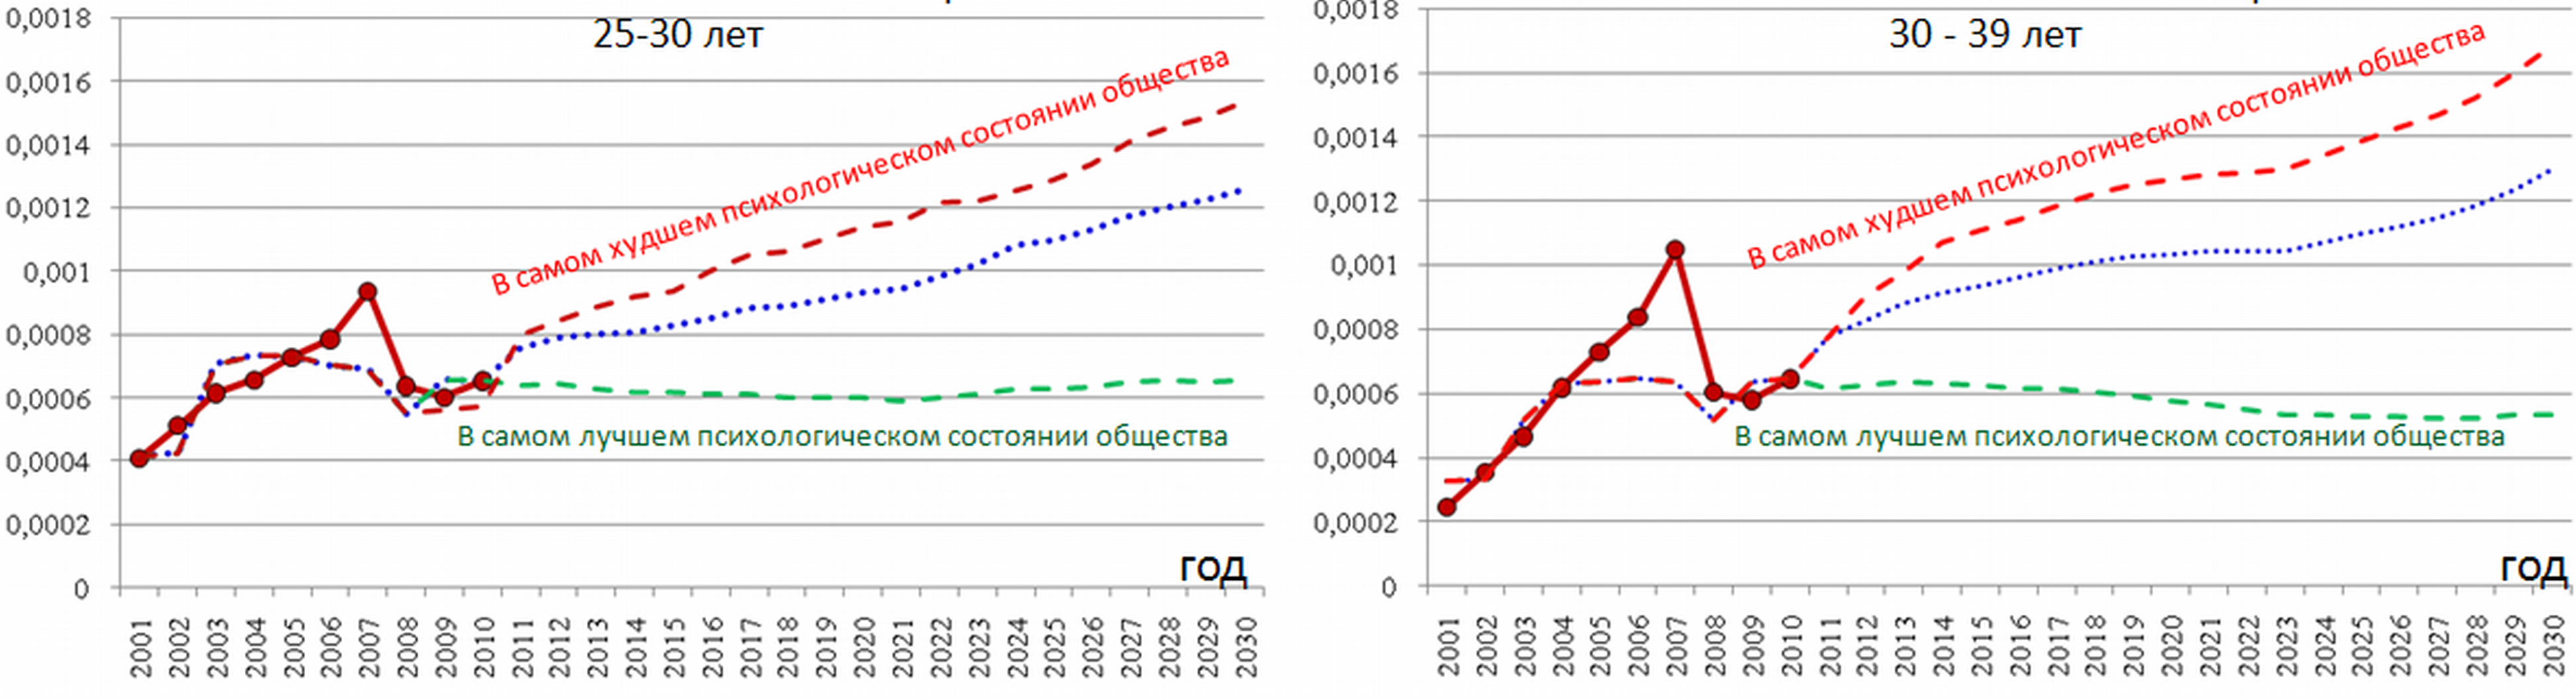
\includegraphics[width=\textwidth]{forecast_emotional.png}
    \caption{Прогнозирование вероятности заболеваемости наркоманией в лучшем и
    худшем эмоционально-психологическом сценарии развития Санкт-Петербурга}
    \label{fig:org_mezhved_antinar}
\end{figure}

Прогнозирование наркоситуации в АИС «Антинар СПб» осуществляется на основе
модуля анализа и ситуационного прогнозирования для автоматизированной
информационной системы мониторинга наркоситуации в Санкт-Петербурге (МАСП АИС
«Антинар СПб»). 

Комплекс предназначен для ситуационного прогнозирования развития наркоситуации
на территории субъекта Федерации. По задаваемым сценариям прогнозируцется
динамика численности наркозависимых с распределением по полу, возрасту и тяжести
заболевания, экономический ущерб от распространения наркомании, демографические
потери от наркомании и снижение демографической устойчивости территории.

Создание автоматизированной информационной системы подразумевает организацию
информационного обмена, как данными, так и документами, что позволяет
унифицировать и упростить взаимодействие между ведомствами и организациями,
участниками мониторинга. И в конечном итоге перейти к информационному
документообороту. 

Но широкий функционал определяет строгие критерии выбора организации,
ответственной за создание и сопровождение автоматизированной информационной
системы, так как ошибка в данном вопросе может привести к развалу всей системы
мониторинга.

В Санкт-Петербурге отлажена система информационного взаимодействия субъектов
антинаркотической деятельности, создана и действует многоуровневая система
профилактики наркомании. Однако, продолжающийся рост незаконного распространения
и немедицинского потребления наркотиков обуславливают необходимость оперативного
реагирования на наркоситуацию всех участников антинаркотической деятельности.
Необходима выработка новых путей и возможностей для повышения эффективности
противодействия наркомании, поднятия уровня доверия населения города к работе
исполнительных органов государственной власти,  правоохранительным и
контролирующим органам. Одним из таких путей является организация комплексного
мониторинга наркоситуации на основе использования современных
информационно-комуникационных технологий.

\section{Сравнение эффективности существующих моделей прогнозирования
наркоситуации с предлагаемой новой моделью на основе нечеткой логики}
текущие модели (из банка): ARIMA, линейный тренд...
[В РАБОТЕ]

